%%%% Paramétrage du TD %%%%
\def\xxactivite{Révisions \ifprof -- Corrigé \else \fi} % \normalsize \vspace{-.4cm}
\def\xxauteur{\textsl{Xavier Pessoles}}


\def\xxnumchapitre{Révision 1 \vspace{.2cm}}
\def\xxchapitre{\hspace{.12cm} Résolution des problèmes de statique -- Modélisation des actions mécaniques}
\def\xxonglet{\textsf{Rév -- Stat}}
\def\xxactivite{Application 01}
\def\xxauteur{\textsl{Xavier Pessoles}}

\def\xxpied{%
Révision statique -- Modélisation des actions mécaniques\\
Fiche 1 -- \xxactivite%
}

\def\xxcompetences{%
\textsl{%
\textbf{Savoirs et compétences :}\\
\vspace{-.3cm}
\footnotesize
\begin{itemize}
\item \textit{Mod2.C20} : modélisation locale, actions à distance et de contact.
\item \textit{Res1.C2.SF1} : proposer une méthode permettant la détermination d’une inconnue de liaison.
\item \textit{Res2.C18} : principe fondamental de la statique.
\item \textit{Res2.C20} : théorème des actions réciproques.
\end{itemize}
\normalsize
}}

\def\xxauteur{\textsl{Xavier Pessoles}}

\def\xxtitreexo{Exercice d'application}
\def\xxsourceexo{\hspace{.2cm} \footnotesize{Xavier Pessoles}}

\def\xxfigures{
%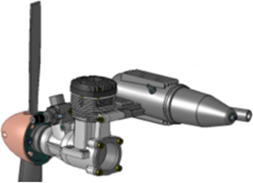
\includegraphics[width=.55\textwidth]{fig_00}
}%figues de la page de garde


\iflivret
\pagestyle{empty}


%%%%%%%% PAGE DE GARDE COURS
\ifcours
% ==== BANDEAU DES TITRES ==== 
\begin{tikzpicture}[remember picture,overlay]
\node at (current page.north west)
{\begin{tikzpicture}[remember picture,overlay]
\node[anchor=north west,inner sep=0pt] at (0,0) {\includegraphics[width=\paperwidth]{\thechapterimage}};
\draw[anchor=west] (-2cm,-8cm) node [line width=2pt,rounded corners=15pt,draw=ocre,fill=white,fill opacity=0.6,inner sep=40pt]{\strut\makebox[22cm]{}};
\draw[anchor=west] (1cm,-8cm) node {\huge\sffamily\bfseries\color{black} %
\begin{minipage}{1cm}
\rotatebox{90}{\LARGE\sffamily\textsc{\color{ocre}\textbf{\xxnumpartie}}}
\end{minipage} \hfill
\begin{minipage}[c]{14cm}
\begin{titrepartie}
\begin{flushright}
\renewcommand{\baselinestretch}{1.1} 
\Large\sffamily\textsc{\textbf{\xxpartie}}
\renewcommand{\baselinestretch}{1} 
\end{flushright}
\end{titrepartie}
\end{minipage} \hfill
\begin{minipage}[c]{3.5cm}
{\large\sffamily\textsc{\textbf{\color{ocre} \discipline}}}
\end{minipage} 
 };
\end{tikzpicture}};
\end{tikzpicture}
% ==== FIN BANDEAU DES TITRES ==== 


% ==== ONGLET 
\begin{tikzpicture}[overlay]
\node[shape=rectangle, 
      rounded corners = .25 cm,
	  draw= ocre,
	  line width=2pt, 
	  fill = ocre!10,
	  minimum width  = 2.5cm,
	  minimum height = 3cm,] at (18.3cm,0) {};
\node at (17.7cm,0) {\rotatebox{90}{\textbf{\Large\color{ocre}{\classe}}}};
%{};
\end{tikzpicture}
% ==== FIN ONGLET 


\vspace{3.5cm}

\begin{tikzpicture}[remember picture,overlay]
\draw[anchor=west] (-2cm,-6cm) node {\huge\sffamily\bfseries\color{black} %
\begin{minipage}{2cm}
\begin{center}
\LARGE\sffamily\textsc{\color{ocre}\textbf{\xxactivite}}
\end{center}
\end{minipage} \hfill
\begin{minipage}[c]{15cm}
\begin{titrechapitre}
\renewcommand{\baselinestretch}{1.1} 
\Large\sffamily\textsc{\textbf{\xxnumchapitre}}

\Large\sffamily\textsc{\textbf{\xxchapitre}}
\vspace{.5cm}

\renewcommand{\baselinestretch}{1} 
\normalsize\normalfont
\xxcompetences
\end{titrechapitre}
\end{minipage}  };
\end{tikzpicture}
\vfill

\begin{flushright}
\begin{minipage}[c]{.3\linewidth}
\begin{center}
\xxfigures
\end{center}
\end{minipage}\hfill
\begin{minipage}[c]{.6\linewidth}
\startcontents
%\printcontents{}{1}{}
\printcontents{}{1}{}
\end{minipage}
\end{flushright}

\begin{tikzpicture}[remember picture,overlay]
\draw[anchor=west] (4.5cm,-.7cm) node {
\begin{minipage}[c]{.2\linewidth}
\begin{flushright}

\includegraphics[width=2cm]{logoCC}
\end{flushright}
\end{minipage}
\begin{minipage}[c]{.2\linewidth}
\textsl{\xxauteur} \\
\textsl{\classe}
\end{minipage}
 };
\end{tikzpicture}

\newpage
\pagestyle{fancy}

%\newpage
%\pagestyle{fancy}

\else
\fi
%% FIN PAGE DE GARDE DES COURS

%%%%%%%% PAGE DE GARDE TD
\iftd
%\begin{tikzpicture}[remember picture,overlay]
%\node at (current page.north west)
%{\begin{tikzpicture}[remember picture,overlay]
%\draw[anchor=west] (-2cm,-3.25cm) node [line width=2pt,rounded corners=15pt,draw=ocre,fill=white,fill opacity=0.6,inner sep=40pt]{\strut\makebox[22cm]{}};
%\draw[anchor=west] (1cm,-3.25cm) node {\huge\sffamily\bfseries\color{black} %
%\begin{minipage}{1cm}
%\rotatebox{90}{\LARGE\sffamily\textsc{\color{ocre}\textbf{\xxnumpartie}}}
%\end{minipage} \hfill
%\begin{minipage}[c]{13.5cm}
%\begin{titrepartie}
%\begin{flushright}
%\renewcommand{\baselinestretch}{1.1} 
%\Large\sffamily\textsc{\textbf{\xxpartie}}
%\renewcommand{\baselinestretch}{1} 
%\end{flushright}
%\end{titrepartie}
%\end{minipage} \hfill
%\begin{minipage}[c]{3.5cm}
%{\large\sffamily\textsc{\textbf{\color{ocre} \discipline}}}
%\end{minipage} 
% };
%\end{tikzpicture}};
%\end{tikzpicture}

%%%%%%%%%% PAGE DE GARDE TD %%%%%%%%%%%%%%%
%\begin{tikzpicture}[overlay]
%\node[shape=rectangle, 
%      rounded corners = .25 cm,
%	  draw= ocre,
%	  line width=2pt, 
%	  fill = ocre!10,
%	  minimum width  = 2.5cm,
%	  minimum height = 2.5cm,] at (18.5cm,0) {};
%\node at (17.7cm,0) {\rotatebox{90}{\textbf{\Large\color{ocre}{\classe}}}};
%%{};
%\end{tikzpicture}

% PARTIE ET CHAPITRE
%\begin{tikzpicture}[remember picture,overlay]
%\draw[anchor=west] (-1cm,-2.1cm) node {\large\sffamily\bfseries\color{black} %
%\begin{minipage}[c]{15cm}
%\begin{flushleft}
%\xxnumchapitre \\
%\xxchapitre
%\end{flushleft}
%\end{minipage}  };
%\end{tikzpicture}

% BANDEAU EXO
\iflivret % SI LIVRET
\begin{tikzpicture}[remember picture,overlay]
\draw[anchor=west] (-2cm,-3.3cm) node {\huge\sffamily\bfseries\color{black} %
\begin{minipage}{5cm}
\begin{center}
\LARGE\sffamily\color{ocre}\textbf{\textsc{\xxactivite}}

\begin{center}
\xxfigures
\end{center}

\end{center}
\end{minipage} \hfill
\begin{minipage}[c]{12cm}
\begin{titrechapitre}
\renewcommand{\baselinestretch}{1.1} 
\large\sffamily\textbf{\textsc{\xxtitreexo}}

\small\sffamily{\textbf{\textit{\color{black!70}\xxsourceexo}}}
\vspace{.5cm}

\renewcommand{\baselinestretch}{1} 
\normalsize\normalfont
\xxcompetences
\end{titrechapitre}
\end{minipage}};
\end{tikzpicture}
\else % ELSE NOT LIVRET
\begin{tikzpicture}[remember picture,overlay]
\draw[anchor=west] (-2cm,-4.5cm) node {\huge\sffamily\bfseries\color{black} %
\begin{minipage}{5cm}
\begin{center}
\LARGE\sffamily\color{ocre}\textbf{\textsc{\xxactivite}}

\begin{center}
\xxfigures
\end{center}

\end{center}
\end{minipage} \hfill
\begin{minipage}[c]{12cm}
\begin{titrechapitre}
\renewcommand{\baselinestretch}{1.1} 
\large\sffamily\textbf{\textsc{\xxtitreexo}}

\small\sffamily{\textbf{\textit{\color{black!70}\xxsourceexo}}}
\vspace{.5cm}

\renewcommand{\baselinestretch}{1} 
\normalsize\normalfont
\xxcompetences
\end{titrechapitre}
\end{minipage}};
\end{tikzpicture}

\fi

\else   % FIN IF TD
\fi


%%%%%%%% PAGE DE GARDE FICHE
\iffiche
\begin{tikzpicture}[remember picture,overlay]
\node at (current page.north west)
{\begin{tikzpicture}[remember picture,overlay]
\draw[anchor=west] (-2cm,-2.25cm) node [line width=2pt,rounded corners=15pt,draw=ocre,fill=white,fill opacity=0.6,inner sep=40pt]{\strut\makebox[22cm]{}};
\draw[anchor=west] (1cm,-2.25cm) node {\huge\sffamily\bfseries\color{black} %
\begin{minipage}{1cm}
\rotatebox{90}{\LARGE\sffamily\textsc{\color{ocre}\textbf{\xxnumpartie}}}
\end{minipage} \hfill
\begin{minipage}[c]{14cm}
\begin{titrepartie}
\begin{flushright}
\renewcommand{\baselinestretch}{1.1} 
\large\sffamily\textsc{\textbf{\xxpartie} \\} 

\vspace{.2cm}

\normalsize\sffamily\textsc{\textbf{\xxnumchapitre -- \xxchapitre}}
\renewcommand{\baselinestretch}{1} 
\end{flushright}
\end{titrepartie}
\end{minipage} \hfill
\begin{minipage}[c]{3.5cm}
{\large\sffamily\textsc{\textbf{\color{ocre} \discipline}}}
\end{minipage} 
 };
\end{tikzpicture}};
\end{tikzpicture}

\iflivret
\begin{tikzpicture}[overlay]
\node[shape=rectangle, 
      rounded corners = .25 cm,
	  draw= ocre,
	  line width=2pt, 
	  fill = ocre!10,
	  minimum width  = 2.5cm,
	  minimum height = 2.5cm,] at (18.5cm,.5cm) {};
\node at (17.9cm,.5cm) {\rotatebox{90}{\textsf{\textbf{\large\color{ocre}{\classe}}}}};
%{};
\end{tikzpicture}
\else
\begin{tikzpicture}[overlay]
\node[shape=rectangle, 
      rounded corners = .25 cm,
	  draw= ocre,
	  line width=2pt, 
	  fill = ocre!10,
	  minimum width  = 2.5cm,
%	  minimum height = 2.5cm,] at (18.5cm,1.1cm) {};
	  minimum height = 2.5cm,] at (18.6cm,0.5cm) {};
\node at (18cm,0.5cm) {\rotatebox{90}{\textsf{\textbf{\large\color{ocre}{\classe}}}}};
%{};
\end{tikzpicture}

\fi

\else
\fi



\else
\pagestyle{empty}


%%%%%%%% PAGE DE GARDE COURS
\ifcours
% ==== BANDEAU DES TITRES ==== 
\begin{tikzpicture}[remember picture,overlay]
\node at (current page.north west)
{\begin{tikzpicture}[remember picture,overlay]
\node[anchor=north west,inner sep=0pt] at (0,0) {\includegraphics[width=\paperwidth]{\thechapterimage}};
\draw[anchor=west] (-2cm,-8cm) node [line width=2pt,rounded corners=15pt,draw=ocre,fill=white,fill opacity=0.6,inner sep=40pt]{\strut\makebox[22cm]{}};
\draw[anchor=west] (1cm,-8cm) node {\huge\sffamily\bfseries\color{black} %
\begin{minipage}{1cm}
\rotatebox{90}{\LARGE\sffamily\textsc{\color{ocre}\textbf{\xxnumpartie}}}
\end{minipage} \hfill
\begin{minipage}[c]{14cm}
\begin{titrepartie}
\begin{flushright}
\renewcommand{\baselinestretch}{1.1} 
\Large\sffamily\textsc{\textbf{\xxpartie}}
\renewcommand{\baselinestretch}{1} 
\end{flushright}
\end{titrepartie}
\end{minipage} \hfill
\begin{minipage}[c]{3.5cm}
{\large\sffamily\textsc{\textbf{\color{ocre} \discipline}}}
\end{minipage} 
 };
\end{tikzpicture}};
\end{tikzpicture}
% ==== FIN BANDEAU DES TITRES ==== 


% ==== ONGLET 
\begin{tikzpicture}[overlay]
\node[shape=rectangle, 
      rounded corners = .25 cm,
	  draw= ocre,
	  line width=2pt, 
	  fill = ocre!10,
	  minimum width  = 2.5cm,
	  minimum height = 3cm,] at (18.3cm,0) {};
\node at (17.7cm,0) {\rotatebox{90}{\textbf{\Large\color{ocre}{\classe}}}};
%{};
\end{tikzpicture}
% ==== FIN ONGLET 


\vspace{3.5cm}

\begin{tikzpicture}[remember picture,overlay]
\draw[anchor=west] (-2cm,-6cm) node {\huge\sffamily\bfseries\color{black} %
\begin{minipage}{2cm}
\begin{center}
\LARGE\sffamily\textsc{\color{ocre}\textbf{\xxactivite}}
\end{center}
\end{minipage} \hfill
\begin{minipage}[c]{15cm}
\begin{titrechapitre}
\renewcommand{\baselinestretch}{1.1} 
\Large\sffamily\textsc{\textbf{\xxnumchapitre}}

\Large\sffamily\textsc{\textbf{\xxchapitre}}
\vspace{.5cm}

\renewcommand{\baselinestretch}{1} 
\normalsize\normalfont
\xxcompetences
\end{titrechapitre}
\end{minipage}  };
\end{tikzpicture}
\vfill

\begin{flushright}
\begin{minipage}[c]{.3\linewidth}
\begin{center}
\xxfigures
\end{center}
\end{minipage}\hfill
\begin{minipage}[c]{.6\linewidth}
\startcontents
%\printcontents{}{1}{}
\printcontents{}{1}{}
\end{minipage}
\end{flushright}

\begin{tikzpicture}[remember picture,overlay]
\draw[anchor=west] (4.5cm,-.7cm) node {
\begin{minipage}[c]{.2\linewidth}
\begin{flushright}

\includegraphics[width=2cm]{logoCC}
\end{flushright}
\end{minipage}
\begin{minipage}[c]{.2\linewidth}
\textsl{\xxauteur} \\
\textsl{\classe}
\end{minipage}
 };
\end{tikzpicture}

\newpage
\pagestyle{fancy}

%\newpage
%\pagestyle{fancy}

\else
\fi
%% FIN PAGE DE GARDE DES COURS

%%%%%%%% PAGE DE GARDE TD
\iftd
%\begin{tikzpicture}[remember picture,overlay]
%\node at (current page.north west)
%{\begin{tikzpicture}[remember picture,overlay]
%\draw[anchor=west] (-2cm,-3.25cm) node [line width=2pt,rounded corners=15pt,draw=ocre,fill=white,fill opacity=0.6,inner sep=40pt]{\strut\makebox[22cm]{}};
%\draw[anchor=west] (1cm,-3.25cm) node {\huge\sffamily\bfseries\color{black} %
%\begin{minipage}{1cm}
%\rotatebox{90}{\LARGE\sffamily\textsc{\color{ocre}\textbf{\xxnumpartie}}}
%\end{minipage} \hfill
%\begin{minipage}[c]{13.5cm}
%\begin{titrepartie}
%\begin{flushright}
%\renewcommand{\baselinestretch}{1.1} 
%\Large\sffamily\textsc{\textbf{\xxpartie}}
%\renewcommand{\baselinestretch}{1} 
%\end{flushright}
%\end{titrepartie}
%\end{minipage} \hfill
%\begin{minipage}[c]{3.5cm}
%{\large\sffamily\textsc{\textbf{\color{ocre} \discipline}}}
%\end{minipage} 
% };
%\end{tikzpicture}};
%\end{tikzpicture}

%%%%%%%%%% PAGE DE GARDE TD %%%%%%%%%%%%%%%
%\begin{tikzpicture}[overlay]
%\node[shape=rectangle, 
%      rounded corners = .25 cm,
%	  draw= ocre,
%	  line width=2pt, 
%	  fill = ocre!10,
%	  minimum width  = 2.5cm,
%	  minimum height = 2.5cm,] at (18.5cm,0) {};
%\node at (17.7cm,0) {\rotatebox{90}{\textbf{\Large\color{ocre}{\classe}}}};
%%{};
%\end{tikzpicture}

% PARTIE ET CHAPITRE
%\begin{tikzpicture}[remember picture,overlay]
%\draw[anchor=west] (-1cm,-2.1cm) node {\large\sffamily\bfseries\color{black} %
%\begin{minipage}[c]{15cm}
%\begin{flushleft}
%\xxnumchapitre \\
%\xxchapitre
%\end{flushleft}
%\end{minipage}  };
%\end{tikzpicture}

% BANDEAU EXO
\iflivret % SI LIVRET
\begin{tikzpicture}[remember picture,overlay]
\draw[anchor=west] (-2cm,-3.3cm) node {\huge\sffamily\bfseries\color{black} %
\begin{minipage}{5cm}
\begin{center}
\LARGE\sffamily\color{ocre}\textbf{\textsc{\xxactivite}}

\begin{center}
\xxfigures
\end{center}

\end{center}
\end{minipage} \hfill
\begin{minipage}[c]{12cm}
\begin{titrechapitre}
\renewcommand{\baselinestretch}{1.1} 
\large\sffamily\textbf{\textsc{\xxtitreexo}}

\small\sffamily{\textbf{\textit{\color{black!70}\xxsourceexo}}}
\vspace{.5cm}

\renewcommand{\baselinestretch}{1} 
\normalsize\normalfont
\xxcompetences
\end{titrechapitre}
\end{minipage}};
\end{tikzpicture}
\else % ELSE NOT LIVRET
\begin{tikzpicture}[remember picture,overlay]
\draw[anchor=west] (-2cm,-4.5cm) node {\huge\sffamily\bfseries\color{black} %
\begin{minipage}{5cm}
\begin{center}
\LARGE\sffamily\color{ocre}\textbf{\textsc{\xxactivite}}

\begin{center}
\xxfigures
\end{center}

\end{center}
\end{minipage} \hfill
\begin{minipage}[c]{12cm}
\begin{titrechapitre}
\renewcommand{\baselinestretch}{1.1} 
\large\sffamily\textbf{\textsc{\xxtitreexo}}

\small\sffamily{\textbf{\textit{\color{black!70}\xxsourceexo}}}
\vspace{.5cm}

\renewcommand{\baselinestretch}{1} 
\normalsize\normalfont
\xxcompetences
\end{titrechapitre}
\end{minipage}};
\end{tikzpicture}

\fi

\else   % FIN IF TD
\fi


%%%%%%%% PAGE DE GARDE FICHE
\iffiche
\begin{tikzpicture}[remember picture,overlay]
\node at (current page.north west)
{\begin{tikzpicture}[remember picture,overlay]
\draw[anchor=west] (-2cm,-2.25cm) node [line width=2pt,rounded corners=15pt,draw=ocre,fill=white,fill opacity=0.6,inner sep=40pt]{\strut\makebox[22cm]{}};
\draw[anchor=west] (1cm,-2.25cm) node {\huge\sffamily\bfseries\color{black} %
\begin{minipage}{1cm}
\rotatebox{90}{\LARGE\sffamily\textsc{\color{ocre}\textbf{\xxnumpartie}}}
\end{minipage} \hfill
\begin{minipage}[c]{14cm}
\begin{titrepartie}
\begin{flushright}
\renewcommand{\baselinestretch}{1.1} 
\large\sffamily\textsc{\textbf{\xxpartie} \\} 

\vspace{.2cm}

\normalsize\sffamily\textsc{\textbf{\xxnumchapitre -- \xxchapitre}}
\renewcommand{\baselinestretch}{1} 
\end{flushright}
\end{titrepartie}
\end{minipage} \hfill
\begin{minipage}[c]{3.5cm}
{\large\sffamily\textsc{\textbf{\color{ocre} \discipline}}}
\end{minipage} 
 };
\end{tikzpicture}};
\end{tikzpicture}

\iflivret
\begin{tikzpicture}[overlay]
\node[shape=rectangle, 
      rounded corners = .25 cm,
	  draw= ocre,
	  line width=2pt, 
	  fill = ocre!10,
	  minimum width  = 2.5cm,
	  minimum height = 2.5cm,] at (18.5cm,.5cm) {};
\node at (17.9cm,.5cm) {\rotatebox{90}{\textsf{\textbf{\large\color{ocre}{\classe}}}}};
%{};
\end{tikzpicture}
\else
\begin{tikzpicture}[overlay]
\node[shape=rectangle, 
      rounded corners = .25 cm,
	  draw= ocre,
	  line width=2pt, 
	  fill = ocre!10,
	  minimum width  = 2.5cm,
%	  minimum height = 2.5cm,] at (18.5cm,1.1cm) {};
	  minimum height = 2.5cm,] at (18.6cm,0.5cm) {};
\node at (18cm,0.5cm) {\rotatebox{90}{\textsf{\textbf{\large\color{ocre}{\classe}}}}};
%{};
\end{tikzpicture}

\fi

\else
\fi



\fi
\setlength{\columnseprule}{.1pt}

\pagestyle{fancy}
\thispagestyle{plain}

\vspace{5cm}

\def\columnseprulecolor{\color{ocre}}
\setlength{\columnseprule}{0.4pt} 

\setcounter{exo}{0}


\ifprof
\begin{multicols}{2}
\else
\begin{multicols}{2}
\fi

\section*{Torseur des actions mécaniques transmissibles dans un coussinet}


\ifprof
\else
Un coussinet (ou bague) est un élément technologique permettant de réaliser des liaisons pivot. Suivant les cas d'utilisation d'un système, un chargement sur l'arbre est transmis au coussinet. 

\begin{center}
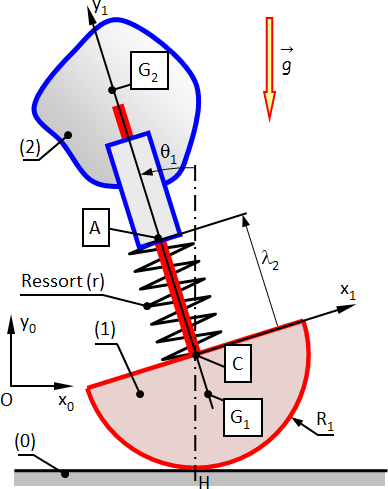
\includegraphics[width=\linewidth]{fig_01}
%\textit{}
\end{center}


On donne le modèle suivant où le champ de pression de l'arbre sur le coussinet est uniforme pour $\theta\in[\pi,2\pi]$ 
On note $R=\dfrac{D}{2}$ le rayon du coussinet. 

\begin{center}
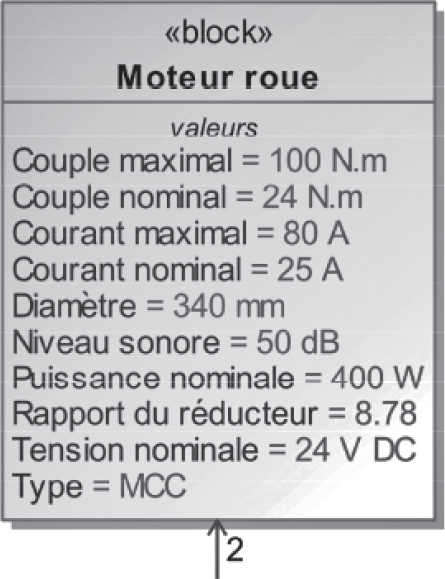
\includegraphics[width=.4\linewidth]{fig_02}
%\textit{}
\end{center}
\fi

\subparagraph{}\textit{Déterminer la résultante des actions mécaniques de 1 sur 3. On la note $\vectf{1}{3}$.}
\ifprof
\begin{corrige}
\begin{enumerate}
\item On commence par exprimer le modèle local d'une action mécanique en $M$ : $\dd \vectf{1}{3} = p(M) \dd S \vect{e_r}$.
\item La pression étant uniforme, on a $p(M)=p$.
\item La géométrie du coussinet étant cylindrique, on se place en coordonnées cylindriques et $\dd S = R\dd \theta \dd z$.  
\item $\theta$ varie sur $[\pi, 2\pi]$ et $z$ sur $[0,L]$. 
\item $\vect{e_r}=\cos\theta\vect{x}+\sin\theta\vect{y}$.
\end{enumerate}
Au final, $\vectf{1}{3}=\int p  \left( \cos\theta\vect{x}+\sin\theta\vect{y}\right)R\dd \theta \dd z$
$=pR\int \left( \cos\theta\vect{x}+\sin\theta\vect{y}\right)\dd \theta \dd z$

$=pR\left( \int  \cos\theta\dd \theta \dd z \vect{x}+\int \sin\theta\dd \theta \dd z   \vect{y}\right)$
$=LpR\left( \int  \cos\theta\dd \theta  \vect{x}+\int \sin\theta\dd \theta   \vect{y}\right)$

$=LpR\left( \left[ \sin \theta \right]^{2\pi}_{\pi}  \vect{x}-\left[\cos \theta \right]^{2\pi}_{\pi}   \vect{y}\right)$

$=LpR\left( -(1-(-1))   \vect{y}\right)$

$=LpR\left( -(1-(-1))   \vect{y}\right)$ $=-2LpR   \vect{y}$ $=-LDp   \vect{y}$.

\end{corrige}
\else
\fi


\subparagraph{}\textit{Déterminer $\vectm{O}{1}{3}\vect{z_N}$.}
\ifprof
\begin{corrige}
\begin{enumerate}
\item On commence par exprimer le modèle local d'une action mécanique en $M$ : $\dd \vectf{1}{3} = p(M) \dd S \vect{e_r}$.
\item Au point $O$, on a $\dd \vectm{O}{1}{3}=\vect{OM}\wedge \dd \vectf{1}{3} =\vect{OM}\wedge \dd \vectf{1}{3} $
\item $\vect{OM}=R\vect{e_r}+z\vect{z}$.
\end{enumerate}
On a alors, $ \vectm{0}{1}{3}\vect{z} =\left( \vect{OM}\wedge \dd \vectf{1}{3}\right) \vect{z}$

$ = \left( \left( R\vect{e_r}+z\vect{z} \right) \wedge  p(M) \dd S \vect{e_r}\right) \vect{z}$

$ = \left(z\vect{z} \wedge  p(M) \dd S \vect{e_r}\right) \vect{z} = 0$


\textbf{Rappel :} le produit mixte est invariant par permutation circulaire : $\left( \vect{a}\wedge \vect{b}\right)\cdot \vect{c} = \left( \vect{c}\wedge \vect{a}\right)\cdot \vect{b} = \left( \vect{b}\wedge \vect{c}\right)\cdot \vect{a}$.
\end{corrige}
\else
\fi

\vspace{.5cm}

On considère maintenant que la pression n'est pas uniforme et vaut au point $M$ $p(M)=p_0\sin\theta$.
\subparagraph{}\textit{Justifier que  $\vectf{1}{3}$ n'a une composante que sur $\vect{y}$.}
\ifprof
\begin{corrige}
Pour des raisons de symétrie du champ de pression, la seule composante sera sur $\vect{y_N}$.
\end{corrige}
\else
\fi


\subparagraph{}\textit{Déterminer la résultante des actions mécaniques de 1 sur 3. On la note $\vectf{1}{3}$. On rappelle que $\sin^2\theta =\dfrac{1-\cos 2\theta }{2}$. }
\ifprof
\begin{corrige}
On cherche donc $\vectf{1}{3} \cdot \vect{y_N}$.
\begin{enumerate}
\item On commence par exprimer le modèle local d'une action mécanique en $M$ : $\dd \vectf{1}{3} = p(M) \dd S \vect{e_r}$.
\item La pression étant uniforme, on a $p(M)=p_0 \sin\theta$.
\item La géométrie du coussinet étant cylindrique, on se place en coordonnées cylindriques et $\dd S = R\dd \theta \dd z$.  
\item $\theta$ varie sur $[\pi, 2\pi]$ et $z$ sur $[0,L]$. 
\end{enumerate}

On a  $\dd \vectf{1}{3} \cdot \vect{y_N} = p(M) \dd S \vect{e_r} \cdot \vect{y_N} =p_0 \dd S  \sin^2 \theta $. 

On a donc $\vectf{1}{3} \cdot \vect{y_N} = \int  p_0  \sin^2 \theta  R\dd \theta \dd z $
$ =   p_0 R L \int \dfrac{1-\cos 2\theta }{2}   \dd \theta$
$ =   \dfrac{1}{2}p_0 R L \left[\theta-\dfrac{1}{2}\sin 2\theta \right]^{2\pi}_{\pi} $
$ =   \dfrac{1}{2}p_0 R L {\pi} $
$ =   \dfrac{1}{4}p_0 D L {\pi} $.
\end{corrige}
\else
\fi

\noindent\footnotesize
\fbox{\parbox{.9\linewidth}{
Éléments de corrigé : 
\begin{multicols}{2}
\begin{enumerate}
 \item $\vectf{1}{3}=-LDp   \vect{y}$.
  \item $\vectm{O}{1}{3}\vect{z_N}=0$.
   \item 
    \item $\vectf{1}{3} \cdot \vect{y_N} =-\dfrac{p_0 D L {\pi} }{4}$.
\end{enumerate}
\end{multicols}}}
\normalsize

\ifprof
\newpage
\else
\fi

\section*{Détermination des efforts dans une structure étayée}
\setcounter{exo}{0}
\ifprof
\else
Lors de la démolition d'une partie de la gare de Lyon Part-Dieu (en 2018), des étais ont du être posés afin de soutenir la structure supérieure. 

\begin{center}
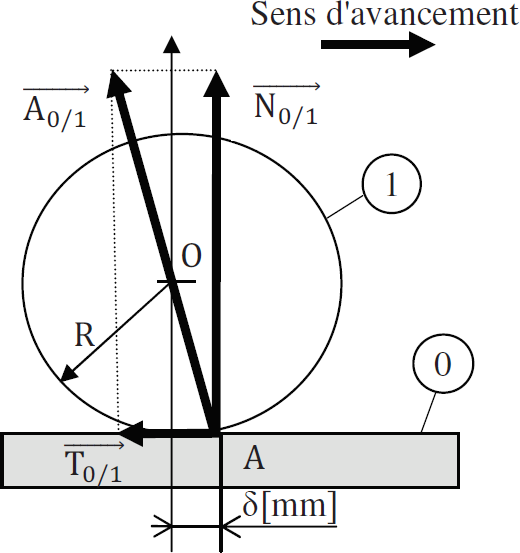
\includegraphics[width=\linewidth]{fig_03}
%\textit{}
\end{center}

Dans le but de dimensionner les étais, il est nécessaire de déterminer les actions mécanique dans chacune des liaisons. 

Pour cela, on utilise la modélisation suivante. 

\begin{center}
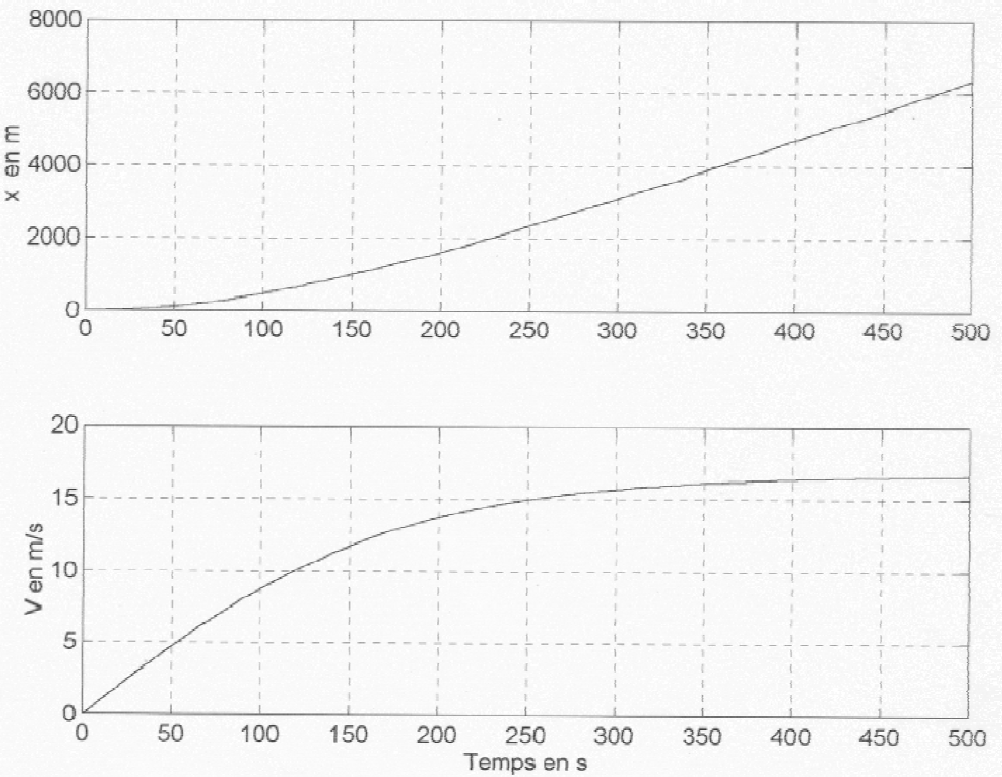
\includegraphics[width=\linewidth]{fig_04}
%\textit{}
\end{center}

On a $\vect{AB}=a \vect{x}$,  $\vect{BD}=b \vect{x}$ et  $\vect{CB}=L \vect{x_1}$.
\fi

\subparagraph{}\textit{Tracer le graphe d'analyse du système (graphe des liaisons et actions extérieures).}
\ifprof
\begin{corrige}
\begin{center}
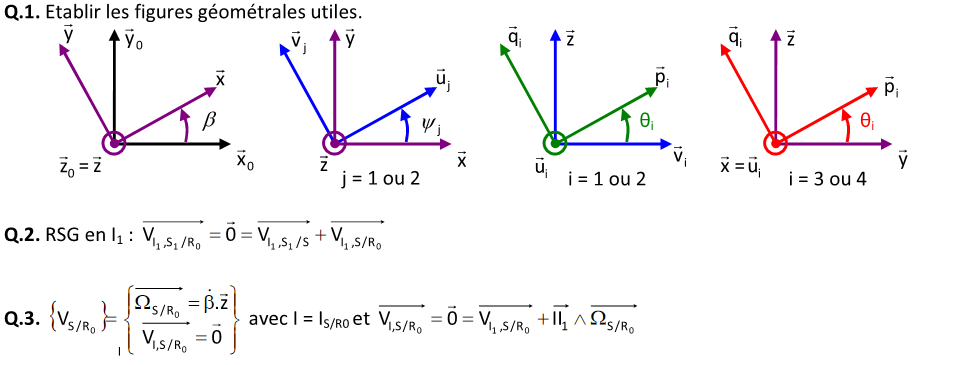
\includegraphics[width=\linewidth]{cor_01}
%\textit{}
\end{center}

\end{corrige}
\else
\fi

\subparagraph{}\textit{Proposer une stratégie permettant de déterminer les actions mécaniques dans les liaisons.}
\ifprof
\begin{corrige}
Ici, il s'agit de déterminer les actions mécaniques dans toutes les liaisons. Il faudra donc isoler successivement toutes les pièces et réaliser un PFS pour chacune d'entre elles. Cependant, il y a quand même une stratégie d'isolement à avoir : \textbf{il faut commencer par isoler les solides soumis à deux glisseurs}. En effet, d'après le PFS, lorsqu'un solide est soumis à deux glisseurs, les deux forces sont de même norme, de même direction (droite passant par le point d'application des deux glisseurs) et de sens opposé. 

La stratégie est donc la suivante : 
\begin{itemize}
\item on isole 1 et on réalise le PFS. 
\item on isole 2 et on réalise le PFS en B. 
\end{itemize} 


\end{corrige}
\else
\fi


\subparagraph{}\textit{Déterminer les actions mécaniques dans les liaisons en fonction de $F$.}
\ifprof
\begin{corrige}

\textbf{On isole 1}.
\textbf{On réalise le BAME :}
\begin{itemize}
\item $\torseurstat{T}{0}{1}$;
\item $\torseurstat{T}{2}{1}$.
\end{itemize}
\textbf{D'après le PFS pour un solide soumis à 2 glisseurs, on a : }
$\torseurstat{T}{0}{1} + \torseurstat{T}{2}{1} = {0}$. 

\textbf{Résolution :} 
$ \torseurstat{T}{0}{1} = -\torseurstat{T}{2}{1}  = \torseurl{F_{01}\vect{x_1}}{\vect{0}}{A}$.

\end{corrige}

\begin{corrige}

\textbf{On isole 2}.
\textbf{On réalise le BAME :}
\begin{itemize}
\item $\torseurstat{T}{0}{2} =\torseurl{X_{02}\vect{x} +Y_{02}\vect{y}  }{\vect{0}}{A} $ $=\torseurl{X_{02}\vect{x} +Y_{02}\vect{y}  }{-aY_{02}\vect{z}}{A} $;
\item $\torseurstat{T}{1}{2} = \torseurl{F_{01}\vect{x_1}  }{\vect{0}}{B} $;
\item $\torseurstat{T}{\text{ext}}{2} = \torseurl{-F\vect{y}  }{\vect{0}}{C} $ $= \torseurl{-F\vect{y}  }{-Fb\vect{z}}{C}$.
\end{itemize}
\textbf{D'après le PFS pour un solide soumis à 2 glisseurs, on a : }

$\torseurstat{T}{0}{2} + \torseurstat{T}{1}{2}+\torseurstat{T}{\text{ext}}{2} = {0}$.

 \textbf{Résolution :}

$\left\{ \begin{array}{l}
X_{02}+F_{01}\cos\alpha  = 0 \\
Y_{02}+F_{01}\sin\alpha  -F= 0 \\
-aY_{02}-Fb  = 0 \\
\end{array}
\right.$


$
\Leftrightarrow 
\left\{ \begin{array}{l}
X_{02}=-F_{01}\cos\alpha  =-F\dfrac{a+b}{a\tan\alpha} \\
F_{01}  =\dfrac{F-Y_{02}}{\sin\alpha}=F\dfrac{a+b}{a\sin\alpha} \\
Y_{02} = -\dfrac{b}{a}F  \\
\end{array}
\right.$

\end{corrige}

\else
\fi


\noindent\footnotesize
\fbox{\parbox{.9\linewidth}{
Éléments de corrigé : 
\begin{enumerate}\setcounter{enumi}{2}
    \item $X_{02}=-F\dfrac{a+b}{a\tan\alpha}$, $F_{01}  =F\dfrac{a+b}{a\sin\alpha}$, $Y_{02} = -\dfrac{b}{a}F$.
\end{enumerate}}}
\normalsize

\ifprof
\end{multicols}
\else
\end{multicols}
\fi
